This interface was used to investigate the possible
route for experimental realization of laser plasma accelerator based coherent
light source (FELs)\cite{Emma2004}. Laser plasma accelerators
(LPA)\cite{Leemans2006,Esarey2009,Tajima1979} have the potential to become the next
generation of accelerator facilities reaching field gradients of the order of
\SI{100}{\giga\electronvolt\per\metre}, i.e. up to three orders of magnitude
higher than in conventional linear accelerators. This would reduce construction
and operation costs by comparable orders of magnitude.

\subsection{Start--to--end simulation of LWFA based FELs\label{sec:lwfa_s2e}}
Our simulation setup is shown in Fig.~\ref{fig:lwfa-setup}; starting from electron
beam generation from a laser plasma source to the generation of femtosecond
and/or attosecond EUV/XUV pulse from the radiation undulator.
%
\begin{figure}[ht]
  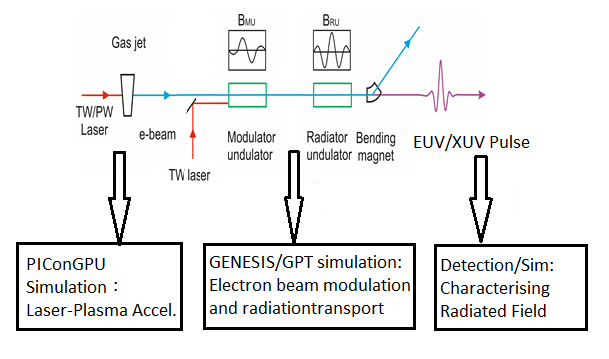
\includegraphics[width=5.4165in,height=2.7374in]{figures/lwfafel-img001.png}
  \caption{Scheme of LWFA-FEL simulation}
  \label{fig:lwfa-setup}
\end{figure}
%
In this scheme an intense
\SIrange{10}{100}{\tera\watt}
laser is focused onto a gas jet or a gas filled capillary for producing a
relativistic electron beam. Initial energy spread of the electron beam of a
LPA (1-5\%) is typically much larger than that of a LINAC (about 0.05 \%), so
reduction of the slice energy spread is necessary. The electron beam is sent
through a modulator undulator (MU) together with a TW-power laser beam, where
the interaction between the electrons, the magnetic field of the undulator and
the electromagnetic field of the laser introduces a periodic energy modulation
of the electrons. This energy modulation leads to the formation of nanobunches
(ultrashort electron layers). The nanobunched electron beam then passes through
a radiator undulator (RU) consisting of a single or a few periods and creates
EUV/XUV pulses.
%
\begin{figure}[ht]
  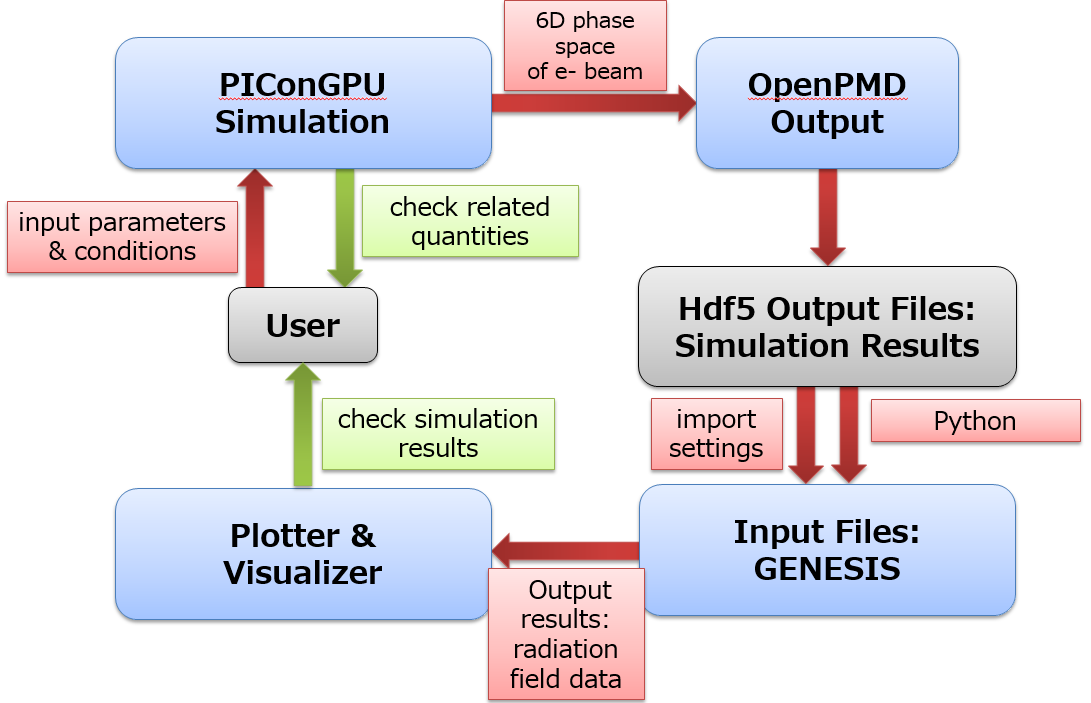
\includegraphics[width=5.9425in,height=4.1882in]{figures/lwfafel-img002.png}
  \caption{Layout for Simulation Setup}
  \label{fig:lwfa-simulation_loop}
\textbf{Need to mention and describe this figure in the text}
\end{figure}
%
\subsection{Laser-plasma accelerator based single-cycle attosecond undulator source}
In parallel, we have studied\footnote{This study was performed in collaboration
with T. Zoltan and Prof. Hebling, both at Pecs University, Hungary.} the feasability of a LWFA based coherent light
source using experimental data for electron wakefield acceleration as input to
the FEL simulation. The FEL simulation used the code \textit{GPT} in this case.
Details are discussed in Ref.~\cite{Tibai2017}.
%
\begin{figure}[ht]
  \centering{%
    \subfloat[]{
      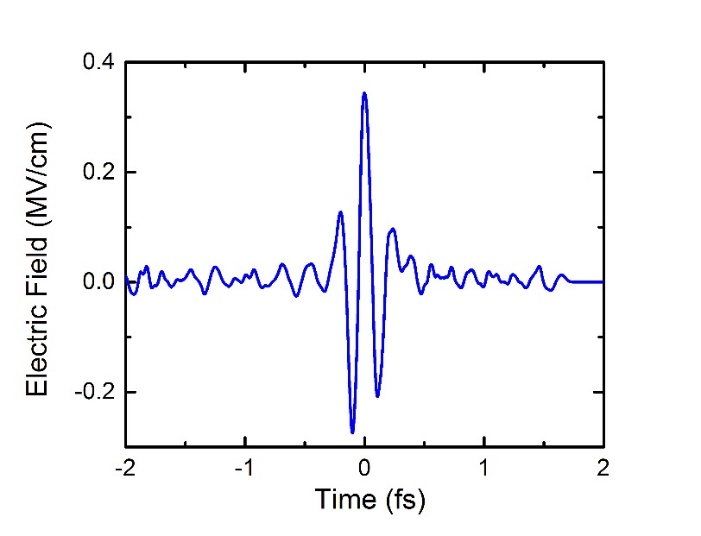
\includegraphics[width=2.7016in,height=2.1583in]{figures/lwfafel-img003.jpg}
      \label{fig:Tibai2017_E_vs_t}
    }
    \subfloat[]{
      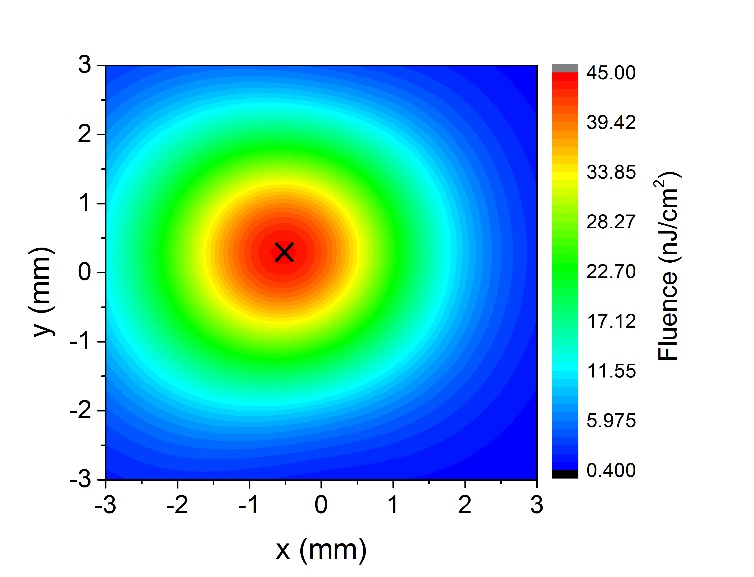
\includegraphics[width=3.0083in,height=2.352in]{figures/lwfafel-img004.jpg}
      \label{fig:Tibai2017_profile}
    }
  }
  \caption{GPT Simulation Results: CEP-controlled EUV waveforms (left) and its spatial beam
    profile (right).\textbf{What is CEP? explain in text}}
    \label{fig:Tibai2017}
\end{figure}
%
Fig.~\ref{fig:Tibai2017} displays the simulated waveform (electric field as
a function of time)  of the generated attosecond
pulse and the beam profile at \SI{60}{\nano\metre} radiation wavelength. The
temporal evolution was measured on the axis of highest intensity, marked by  a
cross in Fig.~\ref{fig:Tibai2017_profile}. In other
wavelengths the shape of the attosecond pulses are nearly identical with the
shape shown in Fig.~\ref{fig:Tibai2017_E_vs_t}, showing that these pulses are
carrier--envelope--phase (CEP) controlled \cite{Tibai2017}.

